\section{قابل مشاهده بودن در مقیاس بزرگ} 
در هنگام تصور سازمانی به بزرگی \lr{Uber} یکی از نیاز‌های مهم قابلیت مشاهده و مانیتورینگ بسیاری از نیاز‌های کیفی همراه با رشد و گسترش سازمان است. برای حفظ ثبات در معماری میکروسرویس دامنه‌گرا که در بخش \cite{domainmicroservice} به آن اشاره شد تیم مشاهده\LTRfootnote{Obserability team} شرکت \lr{Uber} اقدام به ساخت خط لوله‌هایی به منظور تشخیص، هشدار و کاهش عواقب مشکلات در میکروسرویس‌های ساخته‌شده در تیم‌های مهندسی مختلف کرده‌است؛ به عنوان مثال دو نمونه از این خط لوله‌ها به جهت مراقبت از دیتاسنتر‌ها با نام‌های \lr{uMonitor} و \lr{Neris} ساخته شده اند.\lr{uMonitor} سیستم هشدار مبتنی بر معیار‌ها در \lr{Uber} است که بر اساس پلتفرم \lr{M2} \cite{m3_uber} مراکز داده را بررسی می‌کند، در حالی که \lr{Neris} در درجه اول به دنبال هشدارها در زیرساخت های سطح میزبان است.

\section{مدیریت منابع در \lr{Uber}}
یکی زیرساخت‌های نرم افزاری رایج در بین شرکتهای فناوری کلاستر\LTRfootnote{cluster} ها هستند.کلاستر مجموعه‌ای از منابع با میزبان‌های فیزیکی متفاوت است که با تبدیل به یک منبع مشترک منطقی در جهت تقویت توان محاسباتی و استفاده انعطاف پذیر از سخت افزار مراکز داده فعالیت می‌کند. در \lr{Uber}، مدیریت کلاسترها یک لایه انتزاعی برای کارهای مختلف فراهم می کند\cite{resource_uber}.

با افزایش گستره تجارت \lr{Uber} استفاده کارآمد از منابع کلاستر‌ها بسیار مهم می شود.پشته محاسباتی \lr{Uber} به دلیل وجود کلاستر های اختصاصی برای موارد استفاده دسته‌ای\LTRfootnote{Batch} ، باوضعیت\LTRfootnote{Stateful} و بی‌وضعیت\LTRfootnote{Stateless} به مدیریت ویژه‌ای نیازمند است و همچنین ماهیت دینامیک کسب‌و‌کار \lr{Uber} این مساله را سخت‌تر نیز می‌سازد؛ به عنوان مثال دامنه تقاضا برای سفرها با توجه به تعطیلات و ایام هفته بسیار متغیر است.هر چند \lr{Uber} سعی کرده است تا با فراهم آوردن سخت‌افزار بیش از حد نیاز تا جای ممکن در پاسخ به نیاز مشتریان کاستی نداشته باشد اما گاهی در هنگام اوج بار یک محصول و خط کسب‌و‌کار، درست در زمانی که بخشی از کلاستر‌ها اضافه بار دارند، کلاستر سایر محصولات ممکن است فضای خالی بدون استفاده داشته باشند و این تکیه بر کلاستر‌های اختصاصی نیز به این معنی است که \lr{Uber} نمی‌تواند منابع محاسبه ای را بین آنها به اشتراک بگذارد.


برای استفاده بهتر از منابع،\lr{Uber} باید این بارهای کاری را در یک سیستم مدیریت بار واحد محاسبه کند. افزایش کارایی‌های حاصل باعث کاهش هزینه فنی هر سفر در زیرساخت های \lr{Uber} می‌شود و باعث افزاش حاشیه سود سفر‌ها در \lr{Uber} و درنهایت به نفع رانندگان و مسافران خواهد شد.

راه حلی که \lr{Uber} برای مدیریت کلاستر ها ارائه کرده است نرم‌افزار مدیریت یکپارچه کلاستر ها به نام \lr{Peloton} است\cite{resource_uber}؛ \lr{Peloton} یک برنامه‌ریز یکپارچه است که برای مدیریت منابع در بارهای متمایز طراحی شده است و مدیریت کلاستر ها در \lr{Uber} را تجمیع می‌کند. \lr{Peloton} با استفاده از یک پلتفرم مشترک، توازن در استفاده از منابع، به اشتراک گذاری گسترده منابع و پیش‌بینی استفاده از منابع برای نیازهای آینده در \lr{Uber} را پشتیبانی می‌کند.

از سایر محصولات مشابه با \lr{Peloton} می‌توان به \lr{Google Borg}\cite{verma2015large} ،\lr{kubernetes}\cite{kubernetes} ، \lr{Hadoop YARN}\cite{hadoop} و \lr{Apache Mesos/Aurora}\cite{aurora}\cite{mesos} اشاره کرد.

\section{منابع ذخیره‌سازی داده در \lr{Uber}}
پیش از سال ۲۰۱۶ شرکت \lr{Uber} از پایگاه داده \lr{Postgres} استفاده می‌کرد \cite{migration_postgres}، اما امروز با استفاده از روشی بدون طرح\LTRfootnote{Schemaless}\cite{schemaless}  با ترکیب تکنولوژی‌هایی نظیر \lr{Riak}\cite{riak} و \lr{cassandra}\cite{cassandra} به همراه \lr{MySql} داده‌هایی که برای طولانی مدت نیاز به نگهداری دارند، را ذخیره سازی می‌کند.در طول زمان \lr{Postgres} و \lr{Mysql} جای خود را به موتور‌‌های \lr{Nosql} دادند و همچنین به جهت دست‌یابی هر چه بهتر به ویژگی کیفی کارایی در بسیاری از کاربرد ها با افزایش حجم داده‌ها \lr{Riak} جایگاه خود را به \lr{cassandra} می‌دهد.مهندسانی که ابزارهای کاربردی و چند منظوره را برای پذیرش در سراسر \lr{Uber} ایجاد می کنند،از \lr{Cassandra} و \lr{Go} با شدت بیشتری نسبت به تیم های دیگر در \lr{Uber} استفاده می‌کنند که دلیل اصلی آن سرعت است.همچنین \lr{Uber} از \lr{Redis}\cite{redis} هم برای ذخیره سازی داده در حافظه‌های سریع و هم برای صف بندی استفاده می کند و با استفاده از \cite{Twemproxy}\lr{Twemproxy} مقیاس پذیری لایه حافظه پنهان را بدون از بین بردن نسبت برخورد\LTRfootnote{Hit Ratio} حافظه نهان از طریق الگوریتم هش کردن سازگار فراهم می کند.

برای ذخیره سازی توزیع شده و تجزیه و تحلیل داده های پیچیده ،از انبار داده \lr{Hadoop}\cite{hadoop} به جهت ذخیره بهینه داده ها استفاده می‌شود.

\section{ثبت وقایع در \lr{Uber}}
در \lr{Uber}،از \lr{Apache Kafka}\cite{kafka} به عنوان یک گذرگاه پیام برای اتصال قسمت های مختلف اکوسیستم استفاده می‌شود.\lr{Uber} لاگ\LTRfootnote{Log} مربوط به سیستم و برنامه ها و همچنین داده های رویداد را از برنامه های رانندگان و مسافران را جمع آوری می‌کند و سپس این داده‌‌ها را از طریق کافکا\LTRfootnote{Kafka} در دسترس مصرف کنندگان پایین دست قرار می‌دهد.

داده ها در کافکا توسط خطوط لوله \lr{real-time} و خطوط دسته‌ای\LTRfootnote{batch} تغذیه می‌شوند. داده های خطوط لوله مربوط به فعالیت هایی مانند محاسبه معیارهای تجاری ،رفع باگ\LTRfootnote{Bug} ،هشدار و داشبورد است.شکل \ref{fig:kafka} نمایی از نحوه ارتباط کافکا با سایر اجزای معماری رد \lr{Uber} را نشان می‌دهد.\cite{kafka}

\begin{figure}[h]
\centering
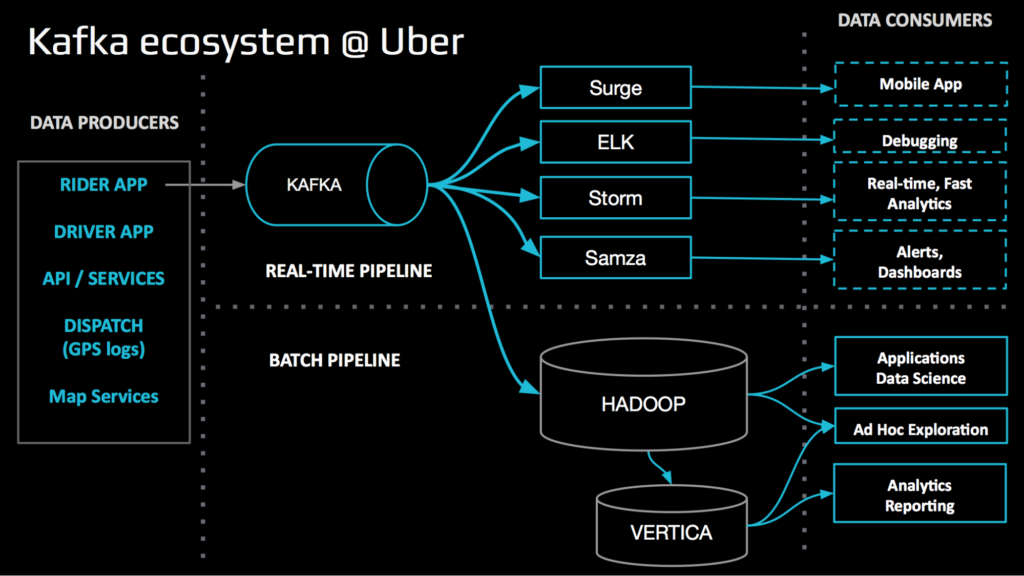
\includegraphics[scale=0.3]{kafka.png}
\caption{کافکا}
\label{fig:kafka}
\end{figure}


\section{تست در \lr{Uber}}
برای اطمینان از اینکه سرویس‌ها قادر به پاسخگویی به تقاضای محیط واقعی هستند، مهندسین در \lr{Uber}  دو نرم افزار \lr{uDestroy} و \lr{Hailstom} را برای تست میکروسرویس‌‌ها ایجاد کرده‌اند.\lr{Hailstorm} تست های ادغام را انجام می‌دهد و زمان اوج بار را نیز شبیه‌سازی می‌کند، در حالی که \lr{uDestroy} عمداً کارها را خراب می کند تا سیستم بتواند در کنترل خرابی های غیر منتظره بهتر عمل کند.

کارمندان \lr{Uber} قبل از اینکه برنامه به دست کاربران برسند، از نسخه بتا برنامه برای آزمایش مداوم تحولات جدید استفاده می کنند و در طی استفاده از نسخه بتا باگ ها را گزارش و ثبت می‌کنند.\cite{techstack}


\section{قابلیت اطمینان و مشاهده‌پذیری در \lr{Uber}}
شرکت \lr{Uber} برای نظارت از سامانه‌ی \lr{Nagios}\cite{Nagios} استفاده می‌کند،که به یک سیستم هشدار برای اعلان‌ها متصل است.در صورتی که کدی در بک‌اند منجر به شکست سیستم شود به مهندسان مربوطه اعلان ارسال می‌شود.

شرکت \lr{Uber} به منظور مانیتورینگ شرایط بخش‌های مختلف سازمان نرم‌افزار \lr{M3}\cite{m3} را گسترش داده است به صورتی که هر سخت افزار و کد توسط این نرم‌افزار تحت نظر قرار دارد.همچنین این شرکت از نرم افزار‌های تشخیص ناهنجاری نظیر \lr{Argos}\cite{argos} برای تشخص ناهنجاری‌ها بر اساس مدلی پیش‌بینی‌کننده مبنی بر داده‌های گذشته استفاده می‌کند که در شکل \ref{fig:argos} نمایی از آن را مشاهده می‌شود.

\begin{figure}[h]
\centering
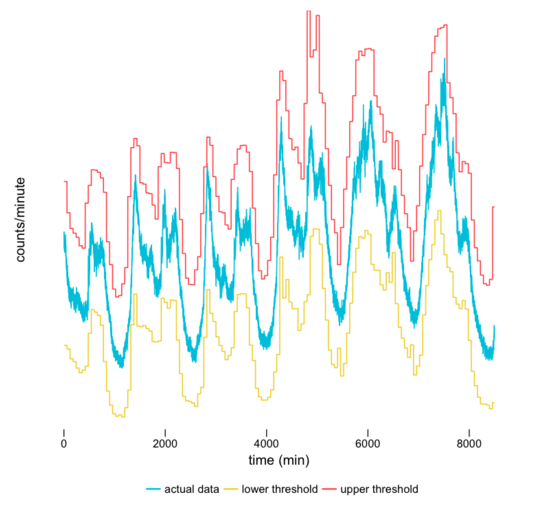
\includegraphics[scale=0.5]{argos.png}
\caption{\lr{Argos}}
\label{fig:argos}
\end{figure}
